\documentclass[border=0.8ex,svgnames,tikz]{standalone}
\usepackage{amsmath,mathtools}
\usepackage{fontspec}
\setmainfont{Source Serif 4}
\setsansfont{Source Sans 3}
\setmonofont{Source Code Pro}
\usetikzlibrary{calc,positioning}
\begin{document}
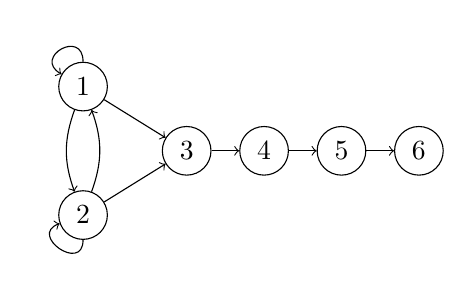
\begin{tikzpicture}
  \node[circle, draw=black](1){1};
  \node[circle, draw=black, below=of 1](2){2};
  \node[circle, draw=black, right=of $(1)!0.5!(2)$](3){3};
  \node[circle, draw=black, right=1em of 3](4){4};
  \node[circle, draw=black, right=1em of 4](5){5};
  \node[circle, draw=black, right=1em of 5](6){6};

  \path[->]
  (1) edge (3)
  (2) edge (3)
  (3) edge (4)
  (4) edge (5)
  (5) edge (6);

  \path[->]
  (1) edge[out=90, in=150, min distance=1.21em] (1)
  (1) edge[out=250, in=110] (2)
  (2) edge[out=270, in=200, min distance=1.21em] (2)
  (2) edge[out=70, in=290] (1);
\end{tikzpicture}
\end{document}
